%Thus far in this work a solution to simplify and automate design the process of all digital PLL loop filter designs comprised of (1) an automated loop filter optimization and design engine, and (2) a discrete-event, time domain PLL simulator to evaluate the designed filters with full time-discretization and quantization nonlinearity effects. I
In this discussion, the performance of the implemented design will first be analyzed via comparison to current state of art.


	\begin{table}[h!]
		\centering
		\def\arraystretch{1.5}		
		\setlength\arrayrulewidth{0.75pt}
		\setlength{\tabcolsep}{1em} % for the horizontal padding
		\begin{tabular}{|c|c|c|c|c|c|}
			\hline 
			\rule[-1ex]{0pt}{2.5ex} \cellcolor{gray!40}\textbf{Parameter} & \cellcolor{gray!40}\textbf{This Work} & \cellcolor{gray!40}\textbf{SSCL 2020}\cite{Liu2020} & \cellcolor{gray!40}\textbf{JSSC 2019}\cite{Liu2019} & \cellcolor{gray!40}\textbf{x} & \cellcolor{gray!40}\textbf{x}\\ 
			\hline 
			\rule[-1ex]{0pt}{2.5ex} \textbf{X} & & & & & \\
			\hline 
		\end{tabular} 
		% \caption{Assigned specifications for branch line hybrid design.}
		% \label{asgn_specs}
		\caption{PLL parameters determined from filter design and optimization process for minimum phase noise with BBPD.}
		\label{tab:state_of_art}
	\end{table}  

\subsection{State of art}
	\begin{figure}[htb!]
	    \centering
	    \begin{subfigure}{0.5\textwidth}
	        \centering
	        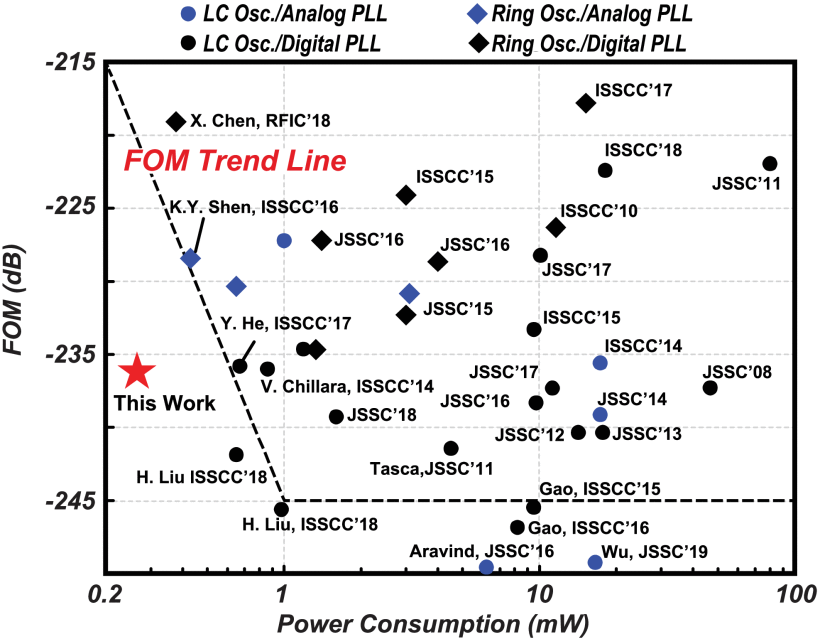
\includegraphics[width=1\textwidth, angle=0]{./figs/liu24-fom}
	        \caption{ }
	        \label{fig:fom_v_pow}
	    \end{subfigure}%
	    \begin{subfigure}{0.5\textwidth}
	        \centering
	        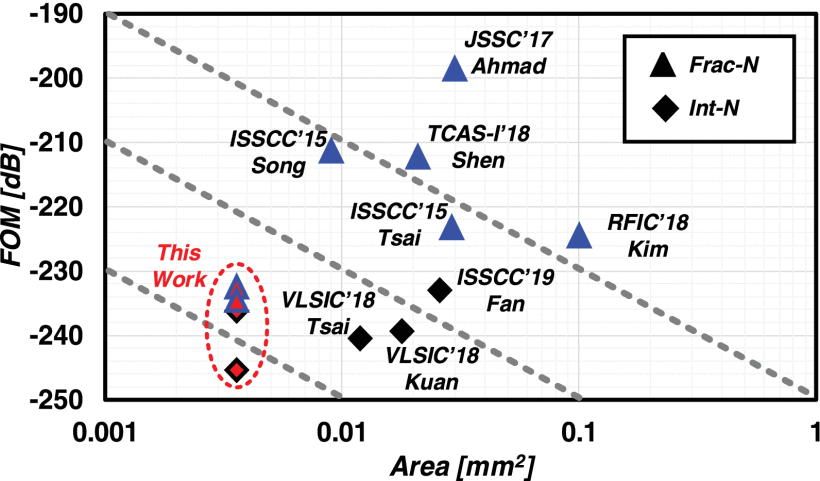
\includegraphics[width=1\textwidth, angle=0]{./figs/liu_5nm}
	        \caption{ }
	        \label{fig:fom_v_area}
	    \end{subfigure}
	    \caption{\textbf{(a)} FOM$_{jitter}$ versus power from \cite{Liu2019} (JSSC 2019), \textbf{(b)} FOM$_{jitter}$ versus area from \cite{Liu2020} (SSCL 2020).}
	    \label{fig:fom_charts}
	\end{figure}


	% \begin{figure}[htb!]
	% 	\center\includegraphics[width=1.0\textwidth, angle=0]{figs/x.pdf}
	% 	\caption{Transient simulation of optimal design.}
	% 	\label{fig:des_ex_trans}
	% \end{figure}
	% \FloatBarrier

	% \begin{figure}[htb!]
	% 	\center\includegraphics[width=1.0\textwidth, angle=0]{figs/x.pdf}
	% 	\caption{Variation Simulation for KDCO.}
	% 	\label{fig:var_lock}
	% \end{figure}
	% \FloatBarrier

	% \begin{figure}[htb!]
	% 	\center\includegraphics[width=1.0\textwidth, angle=0]{figs/x.pdf}
	% 	\caption{Phase noise.}
	% 	\label{fig:Simulated phase noise.}
	% \end{figure}
	% \FloatBarrier

	% stability criteria - Jurys' stability criteria abs(a0) l.t. a2 for second order z-transfer \cite{xiu_li_meiners_padakanti_2004}
	% - Not phase margin based in optimization, can make stable by using stable choice of PI controller (two poles only) - poles should be in unit circle...
\FloatBarrier

\subsection{Areas of improvement}
	\subsubsection{Subharmonic oscillator}
		Possible to be improved to run at full speed, not subharmonic??

	\subsubsection{CDAC switching noise}
		Noise when switching, probably unavoidable with current implementation. Would need other DAC implementation, almost certainly not lower power than CDAC??? 

\FloatBarrier
% \normalsize